En la siguiente sección usaremos el método QR para reducir una matriz tridiagonal simétrica en una matriz similar que es casi diagonal. Las entradas diagonales de la matriz reducida son aproximaciones para los valores propios de la matriz dada. En esta sección presentamos un método concebido por Alston Householder para reducir una matriz simétrica arbitraria en una matriz tridiagonal similar. A pesar de que existe una conexión entre los problemas que estamos resolviendo en estas dos secciones, el método de Householder tiene una aplicación tan amplia en áreas diferentes a la aproximación de valores propios que merece un trato especial.\\
El método de Householder se usa para encontrar una matriz tridiagonal $B$ que es similar a una matriz simétrica $A$ determinada. El teorema 9.16 (\cite{MR2597943}) implica que $A$ es similar a la matriz diagonal $D$, ya que existe una matriz ortogonal $Q$ con la propiedad de que $D=Q^{-1}AQ$. Puesto que, en general, la matriz $Q$ (y por consiguiente, $D$) es difícil de calcular, el método de Householder ofrece un compromiso. Después de haber implementado el método de Householder, es posible usar métodos eficientes, como el algoritmo QR, para aproximar con exactitud los valores propios de la matriz tridiagonal simétrica resultante.
\subsection{Transformaciones de Householder.}
\begin{definition}{}
  Sea $w\in\mathbb{R}^{n}$ con $w^{T}w=1$. Entonces la matriz $n\times n$:
  \begin{align*}
    P=I-2ww^T
  \end{align*}
  recibe el nombre de \textbf{transformación Householder}.
\end{definition}
Las transformaciones de Householder se usan para los bloques externos de entradas cero en vectores o columnas de matrices de manera en extremo estable respecto al error de redondeo. Las propiedades de las transformaciones se dan en el siguiente teorema.
\begin{theorem}{}
  Si una tranformación de Householder, $P=I-2ww^{T}$, es simetrica y ortogonal, entonces $P^{-1}=P$.
\end{theorem}
\begin{proof} 
  Note que
  \begin{align*}
    (ww^{T})^{T}=(w^T)^Tw^T&=ww^T,
  \end{align*}
  luego:
  \begin{align*}
    P^T&=(I-2ww^{T})^T\\
    &=I^{T}-2(ww^{T})^T\\
    &=I-2ww^{T}\\
    &=P.
  \end{align*}
  Además, como $w^{T}w=1$ se satisface que:
  \begin{align*}
    PP^T&=(I-2ww^T)(I-2ww^T)\\
    &=I-2ww^T-2ww^{T}+4ww^Tww^T\\
    &=I-4ww^T+4ww^T &&\text{Ya que $w^Tw=1$.}\\
    &=I.
  \end{align*}
  Así $P^{-1}=P^T=P$.
\end{proof}
El método de Householder comienza determinando una transformación $P^{(1)}$ tal que $A^{(2)}=P^{(1)}AP^{(1)}$ tiene entradas ceros fuera de la primera columna de $A$, comenzando con la tercera fila, es decir:
\begin{equation}\label{eq:m-householder-1}
  a_{j1}^{(2)}=0 \hspace{1cm}\text{Para cada $j=3,4,\cdots,n$.}
\end{equation}
Por simetría también tenemos $a_{1j}^{(2)}=0$.\\
Ahora seleccionamos un vector $w=(w_1,w_2,\cdots,w_n)^{T}$ de tal forma que $w^Tw=1$, la ecuación $\ref{eq:m-householder-1}$ se mantiene y en la matriz:
\begin{align*}
  A^{(2)}&=P^{(1)}AP^{(1)},\\
  &=(I-2ww^T)A(I-2ww^T),
\end{align*}
tenemos $a_{11}^{(2)}=a_{11}$ y $a_{j1}^{(2)}=0$ para cada $j=3,4,\cdots,n$. Esta selección impone $n$ condiciones en los $n$ valores desconocidos $w_1,w_2,\cdots,w_n$.\\
Al establecer $w_1=0$ garantizamos que $a_{11}^{(2)}=a_{11}$. Queremos:
\begin{align*}
  P^{(1)}=I-2ww^T,
\end{align*}
para satisfacer:
\begin{equation}\label{eq:m-householder-2}
  P^{(1)}(a_{11},a_{21},a_{31},\cdots,a_{n1})^{T}=(a_{11},\alpha,0,\cdots,0)^T
\end{equation}
donde $\alpha$ se seleccionará más adelante. Para simplificar la notación, si:
\begin{align*}
  \hat{w}=(w_2,w_3,\cdots,w_n)^{T}\in\mathbb{R}^{n-1}, \hat{y}=(a_{21},a_{31},\cdots,a_{n1})^{T}\in\mathbb{R}^{n-1},  
\end{align*}
y $\hat{P}$ es una transformación de Householder $(n-1)\times(n-1)$:
\begin{align*}
  \hat{P}=I_{n-1}-2\hat{w}\hat{w}^T.
\end{align*}
Entonces la ecuación $\ref{eq:m-householder-2}$ se convierte en:\\
Inserte matrices feas\\ 
con:
\begin{equation}\label{eq:m-householder-9.10}
  \hat{P}\hat{y}=(I_{n-1}-2\hat{w}\hat{w}^T)\hat{y}=\hat{y}-2(\hat{w}^T\hat{y})\hat{w}=(\alpha,0,\cdots,0)^T.
\end{equation}
Sea $r=\hat{w}^T\hat{y}$. Entonces:
\begin{align*}
  (\alpha,0,\cdots,0)^{T}=(a_{21}-2rw_2,a_{31}-2rw_3,\cdots,a_{n1}-2rw_n)^T,
\end{align*}
y podemos determinar todas las $w_i$ una vez que conocemos $\alpha$ y $r$. Al equiparar los componentes da:
\begin{align*}
  \alpha=a_{21}-2rw_2
\end{align*}
y
\begin{align*}
  0=a_{j1}-2rw_j, \hspace{1cm}\text{para cada }j=3,4\cdots,n.
\end{align*}
Por lo tanto:
\begin{equation}\label{eq:m-householder-9.11}
  2rw_2=a_{21}-\alpha,
\end{equation}
y
\begin{equation}\label{eq:m-householder-9.12}
  2rw_j=a_{j1},\hspace{1cm}\text{para cada }j=3,4,\cdots,n.
\end{equation}
Al elevar al cuadrado ambos lados de cada una de las ecuaciones \ref{eq:m-householder-9.11}, \ref{eq:m-householder-9.12} y sumar los términos correspondientes da:
\begin{align*}
  4r^2\sum_{j=2}^{n}w_j^2=(a_{21}-\alpha)^{2}+\sum_{j=3}^{n}a_{j1}^{2}
\end{align*}
note que como $ww^{T}=1$ y $w_1=0$, entonces $\sum_{j=2}^{n}w_{j}^{2}=1$,
\begin{equation}\label{eq:m-householder-9.13}
  4r^{2}=\sum_{j=2}^{n}a_{j1}^{2}-2\alpha a_{21}+\alpha^2.
\end{equation}
La ecuación \ref{eq:m-householder-9.10} y el hecho de que $P$ es ortogonal implica que:
\begin{align*}
  \alpha^2&=(\alpha,0,\cdots,0)(\alpha,0\cdots,0)^{T},\\
  &=(\hat{P}\hat{y})^{T}\hat{P}\hat{y},\\
  &=\hat{y}^{T}\hat{P}^{T}\hat{P}\hat{y},\\
  &=\hat{y}^T\hat{y}.
\end{align*}
Por lo tanto:
\begin{align*}
  \alpha^{2}=\sum_{j=2}^{n}a_{j1}^{2},
\end{align*}
lo que, al sustituir en la ecuación \ref{eq:m-householder-9.13}, da
\begin{align*}
  2r^{2}=\sum_{j=2}^{n}a_{j1}^2-\alpha a_{21}.
\end{align*}
Para garantizar $2r^2=0$ si y sólo si $a_{21}=a_{31}=\cdots=a_{n1}=0$ seleccionamos:
\begin{align*}
  \alpha=-sgn(a_{21})\left( \sum_{j=2}^{n}a_{j1}^{2} \right)^{\frac{1}{2}},
\end{align*}
lo cual implica que:
\begin{align*}
  2r^{2}=\sum_{j=2}^{n}a_{j1}^{2}+|a_{21}|\left( \sum_{j=2}^{n}a_{j1}^{2} \right)^{\frac{1}{2}}.
\end{align*}
Con esta selección de $\alpha$ y $2r^2$, resolvemos las ecuaciones \ref{eq:m-householder-9.11} y \ref{eq:m-householder-9.12} para obtener:
\begin{align*}
  w_{2}=\frac{a_{21}-\alpha}{2r}\text{ y }w_{j}=\frac{a_{j1}}{2r},\text{ para cada }j=3,\cdots,n.
\end{align*}
para resumir la selección de $P^{(1)}$, tenemos:
\begin{align*}
  \alpha&=-sgn(a_{21})\left( \sum_{j=2}^{n}a_{j1}^2 \right)^{\frac{1}{2}},\\
  r&=\left( \frac{1}{2}\alpha^2-\frac{1}{2}a_{21}\alpha \right)^{\frac{1}{2}},\\
  w_1&=0,\\
  w_2&=\frac{a_{21}-\alpha}{2r},
\end{align*}
y
\begin{align*}
  w_{j}=\frac{a_{j1}}{2r},\text{ por cada }j=3,\cdots,n.
\end{align*}
Con esta selección:
\begin{align*}
  A^{(2)}&=P^{(1)}AP^{(1)}\\
  &=\begin{bmatrix}
    a_{11}^{(2)}& a_{12}^{(2)}& 0 & \cdots & 0 \\
    a_{21}^{(2)} & a_{22}^{(2)} & a_{23}^{(2)} & \cdots & a_{2n}^{(2)} \\
    0 & a_{32}^{(2)} & a_{33}^{(2)} & \cdots & a_{3n}^{(2)} \\
    \vdots & \vdots & \vdots &  & \vdots \\
    0 & a_{n2}^{(2)} & a_{n3}^{(2)} & \cdots & a_{nn}^{(2)}
  \end{bmatrix} 
\end{align*}
Al haber cálculado $P^{(1)}$ y calculado $A^{(2)}$, el proceso se repite para $k=2,3,\cdots,n-2$ de acuerdo con lo siguiente:
\begin{align*}
  \alpha&=-sgn(a_{k+1,k}^{(k)})\left( \sum_{j=k+1}^{n}(a_{jk}^{(k)})^{2} \right)^{\frac{1}{2}},\\
  r&=\left( \frac{1}{2}\alpha^2-\frac{1}{2}\alpha\alpha_{k+1,k}^{(k)} \right)^{\frac{1}{2}},\\
  w_1^{(k)}=w_{2}^{(k)}=\cdots=w_{k}^{(k)}=0,\\
  w_{k+1}&=\frac{a_{k+1,k}^{(k)}-\alpha}{2r},\\
  w_{j}^{(k)}=\frac{a_{jk}^{(k)}}{2r},\text{ para cada }j=k+2,k+3,\cdots,n,\\
  P^{(k)}=I-2w^{(k)}\dot(w^{(k)})^T,
\end{align*}
y:
\begin{align*}
  A^{(k+1)}=P^{(k)}A^{(k)}P^{(k)},
\end{align*}
donde
\begin{center}
  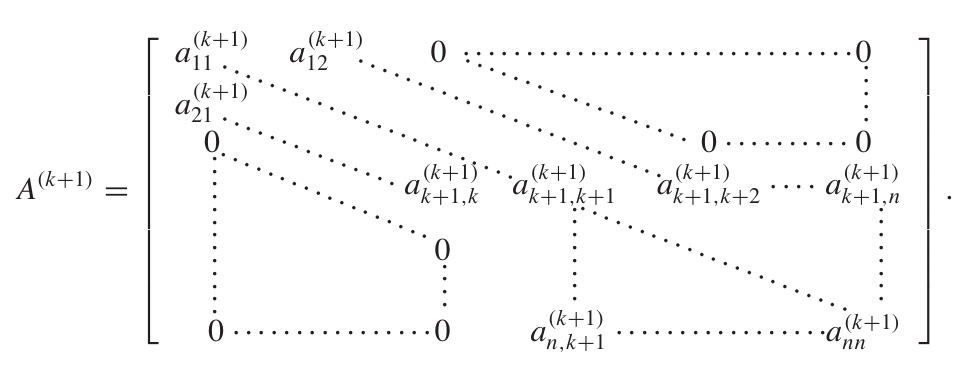
\includegraphics[scale=0.5]{matrizfea.png}
\end{center}
















